\documentclass[11pt]{article}

\usepackage[margin=1in]{geometry}
\usepackage{amsmath}
\usepackage{booktabs}
\usepackage{graphicx}
\usepackage{array}
\usepackage{enumitem}
\usepackage{float}
\usepackage{xcolor}
\usepackage{hyperref}
\usepackage{microtype}
\usepackage{xspace}
\usepackage[T1]{fontenc}
\usepackage{lmodern}

\graphicspath{{../figures/}}
\hypersetup{
  colorlinks=true,
  linkcolor=black,
  citecolor=black,
  urlcolor=blue
}

\setlist[itemize]{leftmargin=1.35em}
\setlist[enumerate]{leftmargin=1.35em}
\setlength{\parskip}{0.35em}
\setlength{\parindent}{0pt}
\emergencystretch=3em

\newcommand{\NL}{\texttt{NL}\xspace}
\newcommand{\MD}{\texttt{MARKDOWN}\xspace}
\newcommand{\JS}{\texttt{JSON}\xspace}
\newcommand{\SM}{\texttt{SHARED\_MEMORY}\xspace}
\newcommand{\RD}{\texttt{RELAY\_DEFAULT}\xspace}
\newcommand{\SMJ}{\texttt{SHARED\_MEMORY\_JSON}\xspace}
\newcommand{\SMN}{\texttt{SHARED\_MEMORY\_NL}\xspace}
\newcommand{\SMM}{\texttt{SHARED\_MEMORY\_MARKDOWN}\xspace}

\title{\textbf{Communication Protocol Effects on Multi-Agent System Efficiency and Task Completion}\\
\large STAT GR5293 Generative AI using Large Language Models}
\author{Yi Zhang (yz5104) \and Xian Zhang (xz3447) \and Tianyu Zhan (tz2704)\\
Department of Statistics, Columbia University}
\date{May 2026}

\begin{document}
\maketitle

\begin{abstract}
Multi-agent LLM systems increasingly rely on specialized agents that pass intermediate plans, evidence, and partial answers to one another. Yet the representation used for that internal communication is usually treated as an implementation detail rather than an experimental factor. We study this factor directly with a fixed three-agent pipeline, Planning $\rightarrow$ Execution $\rightarrow$ Integration, while varying only the inter-agent protocol. The main experiment runs a full $4 \times 3$ factorial grid over four protocols, \NL, \MD, \JS, and \SM, and three domains, GSM8K math, SQuAD reading, and curated news analysis, for 360 pipeline runs and 1,080 agent calls on \texttt{gpt-4o-mini}. Protocol has a large effect on efficiency: a two-way ANOVA attributes $\eta^2=0.262$ of token variance to protocol, with \SM costing 338 more tokens per run than \NL on average. Effectiveness is domain-dependent: protocol is not significant for math, but \SM improves reading and news completion despite its overhead. Supplemental ablation and DeepSeek V4 Flash robustness runs increase the total logged scope to 960 pipeline runs and show that blackboard-style shared state reliably increases token cost, while quality rankings remain model- and domain-specific.
\end{abstract}

\section{Introduction}

Multi-agent LLM systems have moved from research prototypes into practical tools for coding, research assistance, retrieval, planning, and enterprise workflow automation. Frameworks such as LangGraph, AutoGen, and CrewAI make it easy to compose specialized agents into graphs or conversations, where one agent plans, another executes, and a final agent integrates the result \cite{langgraph, autogen, crewai}. As these systems grow, the internal communication format becomes consequential: an intermediate message can preserve evidence, impose structure, inflate context length, or silently lose information.

Despite this practical importance, protocol choice is rarely studied systematically. Most agentic systems papers ask what a multi-agent system can accomplish. This project asks a lower-level design question: holding the agents and tasks fixed, how does the representation of inter-agent communication change cost, latency, and completion quality? This protocol-level focus is the main differentiator of the project. We do not propose a new task-specific agent application; instead, we treat the multi-agent pipeline itself as the experimental object.

The study is organized around two research questions:

\begin{itemize}
  \item \textbf{RQ1, efficiency.} How do different inter-agent communication protocols compare in token consumption and response latency across task domains?
  \item \textbf{RQ2, effectiveness.} How does protocol choice interact with task domain to affect task completion quality? Is there a universally optimal protocol, or does the best choice depend on domain?
\end{itemize}

The two questions are linked. The cheapest protocol may not preserve enough information for later agents, while the most faithful protocol may be too expensive for routine use. Our goal is to characterize this trade-off and produce protocol-selection guidelines for practitioners building multi-agent systems.

The project makes four contributions. First, it provides a controlled multi-domain comparison of inter-agent communication protocols. Second, it turns the results into practical guidance for systems built with LangGraph, AutoGen, CrewAI, or similar frameworks. Third, it applies classical statistical tools, including two-way ANOVA, Tukey HSD, Cohen's $d$, and bootstrap confidence intervals, to an LLM systems question. Fourth, it releases reusable artifacts: the experiment framework in \texttt{pipeline.py}, result tables and message logs under \texttt{results/}, figures under \texttt{figures/}, and a FastAPI dashboard in \texttt{fastapi\_app.py} plus \texttt{dashboard/}.

\section{Related Work}

\textbf{Multi-agent LLM frameworks.} LangGraph offers graph-structured orchestration for stateful multi-actor LLM applications \cite{langgraph}. AutoGen formalizes multi-agent conversation patterns and has become a common research platform for collaborative LLM workflows \cite{autogen}. CrewAI popularizes role-based agent teams with task delegation and workflow abstractions \cite{crewai}. These frameworks make protocol design configurable, but they generally do not prescribe which message representation should be used between agents. Our study treats that open engineering choice as the independent variable.

\textbf{Agent communication and structured output.} Structured generation has been studied in tool-use and constrained-decoding settings. Toolformer showed that language models can learn to call tools using generated annotations \cite{toolformer}. Guided generation and constrained decoding methods reduce malformed structured output by limiting the token space during decoding \cite{guided}. AgentVerse explores collaborative multi-agent behavior, but does not isolate communication format as a controlled factor across task domains \cite{agentverse}. Our study differs by treating format not as a parser convenience for one output, but as a repeated communication protocol across a three-agent pipeline.

\textbf{Multi-agent evaluation.} AgentBench evaluates LLM agents in diverse interactive environments and emphasizes systematic benchmarking of agent capabilities \cite{agentbench}. Multi-agent debate studies show that communication among agents can improve factuality or reasoning in some settings \cite{debate}. However, these evaluations usually hold the communication style fixed. We instead vary the protocol while holding the model, roles, task inputs, and evaluation functions fixed.

\textbf{Task-specific LLM performance.} GSM8K evaluates grade-school mathematical reasoning with numeric answers \cite{gsm8k}. SQuAD evaluates extractive reading comprehension with token-level exact match and F1 \cite{squad}. ROUGE remains a standard automatic metric family for summarization and information recall \cite{rouge}, and information extraction surveys document the difficulty of measuring fact preservation in text outputs \cite{ie}. These benchmarks motivate our domain selection: math, reading, and news analysis stress different answer types and error modes. We ask whether those domain differences interact with communication protocol inside a multi-agent system.

\section{Methodology}

\subsection{System Model}

We model a multi-agent pipeline as a directed chain of three LLM-backed agents:

\[
\text{Planning Agent} \rightarrow \text{Execution Agent} \rightarrow \text{Integration Agent}.
\]

The Planning Agent decomposes the task into subtasks, the Execution Agent solves or extracts the requested information, and the Integration Agent produces the final answer. Agent roles, system prompts, model, temperature, task text, and maximum output length are held constant across protocol conditions. The sole manipulated factor in the main experiment is the communication protocol used for intermediate agent outputs.

The implementation is centralized in \texttt{pipeline.py}. The base model is \texttt{gpt-4o-mini}, temperature is 0.3, and maximum output lengths are 256 tokens for math and reading and 512 tokens for news. Each repetition uses the OpenAI \texttt{seed} parameter with the repetition index, plus Python and NumPy seeding where sampling is used. The logger records one message per agent call with sender, receiver, content, prompt tokens, completion tokens, total tokens, latency, finish reason, JSON parse status, protocol, domain, and run ID.

All token counts come from the provider usage fields returned by each agent call, not from a local tokenizer estimate. Latency is measured as wall-clock elapsed time around the API call and then summed across the three agents in a run. A run is marked as truncated if any agent response returns \texttt{finish\_reason=length}; this is the definition used later in the error analysis.

\subsection{Protocols}

The main experiment compares four protocols:

\begin{itemize}
  \item \NL: explicit plain English prose, with instructions not to use markdown, bullets, headings, JSON, or other structured formatting.
  \item \MD: semi-structured output with markdown headings, bullets, and numbered lists.
  \item \JS: valid JSON objects with descriptive field names, enforced with OpenAI structured response formatting and one parse-validate-retry.
  \item \SM: a shared blackboard. Every downstream agent receives a serialized JSON snapshot of the accumulated global state, not merely the predecessor's last message.
\end{itemize}

Two implementation details are important for internal validity. First, \SM is a true shared-state mechanism: the integrator sees the original task, the plan, and the execution result through the blackboard snapshot. This makes the expected overhead of shared memory testable. Second, \NL uses an explicit anti-markdown instruction. Without that instruction, \texttt{gpt-4o-mini} tends to produce lightly structured bullet-point output, which would contaminate the contrast between \NL and \MD.

The shared-memory prompt injects a serialized JSON snapshot under a \texttt{BLACKBOARD STATE} block before the agent's role-specific task. After the planner writes the plan, the executor reads the full snapshot and writes execution results; the integrator then reads the accumulated task, plan, and execution result. For \JS, the API is called with structured JSON response formatting. If parsing fails, the call is retried once with the same role and task context; only a second failure is logged as an unrecoverable JSON parse error.

\subsection{Task Domains and Evaluation}

The design uses three domains with distinct answer forms:

\begin{itemize}
  \item \textbf{Math, GSM8K.} Grade-school word problems with a single numeric answer. Evaluation is exact numeric match, scored 0 or 1.
  \item \textbf{Reading, SQuAD.} Extractive question answering over passages. Evaluation is SQuAD-style token-level F1 against gold answer spans.
  \item \textbf{News analysis.} Ten curated news articles with manually reviewed key facts. Evaluation is the mean of ROUGE-2 F1 and ROUGE-L F1 against the concatenated key-facts reference.
\end{itemize}

These evaluators were chosen to avoid common false positives. Substring matching can incorrectly reward negated answers, and simple keyword overlap can reward summaries that mention entities while reversing facts. The self-tests embedded in \texttt{pipeline.py} check representative negation cases and can be run with \texttt{python pipeline.py}.

\subsection{Experimental Design}

The main experiment is a full $4 \times 3$ factorial design:

\[
4\ \text{protocols} \times 3\ \text{domains} \times 10\ \text{samples per domain} \times 3\ \text{repetitions} = 360\ \text{pipeline runs}.
\]

Each run has three agent calls, so the main experiment records 1,080 message-level observations. The committed result files are \texttt{results/results\_raw.csv}, \texttt{results/results\_messages.jsonl}, \texttt{results/results\_summary.csv}, and \texttt{results/experiment\_config.json}.

Two supplemental experiment sets are included in the latest repository outputs. A full mechanism-format ablation adds 360 runs for \RD, \SMN, \SMM, and \SMJ. This separates the relay-vs-blackboard mechanism from output format. A DeepSeek V4 Flash robustness check adds 240 runs over all eight protocols with five samples per domain and two repetitions. These supplemental outputs are used as robustness evidence, while the primary inferential claims remain anchored in the proposal-defined 360-run \texttt{gpt-4o-mini} grid.

\subsection{Statistical Analysis}

For token cost, latency, and completion score, we fit two-way ANOVA models with protocol, domain, and protocol-by-domain interaction terms. For completion score, pooled ANOVA is interpreted cautiously because the metric has different semantics across domains: binary exact match for math and continuous overlap scores for reading and news. Therefore, primary effectiveness interpretation is based on per-domain one-way ANOVA, Tukey HSD post-hoc comparisons, and effect sizes. Bootstrap percentile confidence intervals with 2,000 resamples summarize uncertainty in cell means.

For token cost, the pooled Tukey HSD is used as a descriptive main-effect ranking across the full grid. Because the token ANOVA also finds a significant protocol-by-domain interaction, domain-level cell means and confidence intervals are used for protocol recommendations rather than relying on the pooled ranking alone.

\section{Results}

\subsection{RQ1: Efficiency}

Protocol choice strongly affects token cost. Table~\ref{tab:anova} reports Type II two-way ANOVA results for total tokens, latency, and completion score in the main 360-run grid.

\begin{table}[H]
\centering
\caption{Two-way ANOVA results for the main experiment. $\eta^2$ is computed against total sum of squares.}
\label{tab:anova}
\begin{tabular}{llrrr}
\toprule
Metric & Term & F & p-value & $\eta^2$ \\
\midrule
Total tokens & Protocol & 87.40 & $<0.001$ & 0.262 \\
Total tokens & Domain & 148.19 & $<0.001$ & 0.296 \\
Total tokens & Protocol $\times$ Domain & 15.66 & $<0.001$ & 0.094 \\
\midrule
Latency & Protocol & 16.55 & $<0.001$ & 0.070 \\
Latency & Domain & 136.44 & $<0.001$ & 0.385 \\
Latency & Protocol $\times$ Domain & 6.38 & $<0.001$ & 0.054 \\
\midrule
Completion & Protocol & 2.36 & 0.071 & 0.012 \\
Completion & Domain & 125.42 & $<0.001$ & 0.408 \\
Completion & Protocol $\times$ Domain & 1.43 & 0.203 & 0.014 \\
\bottomrule
\end{tabular}
\end{table}

The token ANOVA shows that protocol explains 26.2\% of token variance and that protocol efficiency depends on domain. Tukey HSD on pooled token cost finds all six pairwise protocol comparisons significant at family-wise $\alpha=0.05$. The mean ordering from cheapest to most expensive is:

\[
\NL \prec \JS \prec \MD \prec \SM.
\]

\SM costs 337.6 more tokens per run than \NL on average. \MD costs 224.0 more tokens than \NL, while \JS costs 104.3 fewer tokens than \NL in the pooled contrast. This supports the main overhead hypothesis for shared memory, but qualifies the original expectation that JSON would always be cheapest: JSON is cheapest for math, while \NL is cheapest for reading and news.

\begin{figure}[H]
\centering
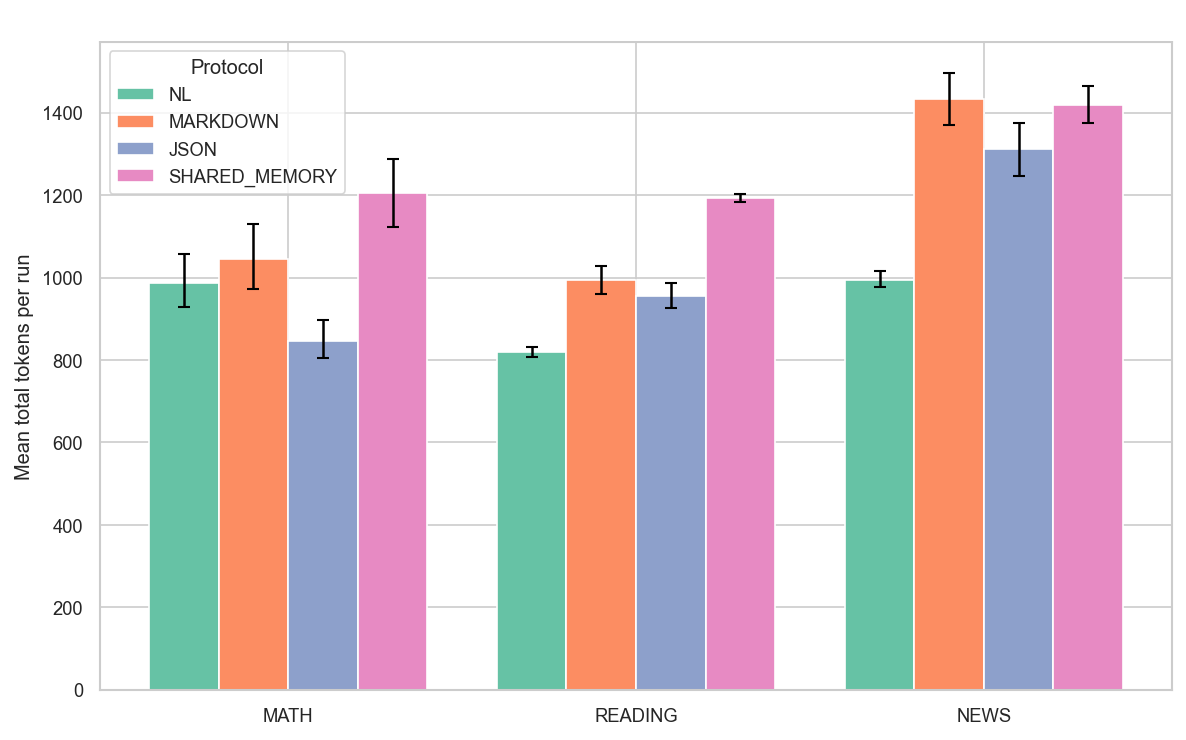
\includegraphics[width=0.96\linewidth]{report_fig1_tokens_by_protocol_domain.png}
\caption{Mean total tokens by protocol and domain. Shared Memory is consistently expensive, while the cheapest protocol is domain-dependent.}
\label{fig:tokens}
\end{figure}

The cell-level means in Table~\ref{tab:summary} show the mechanism behind this result. Shared memory increases prompt tokens because the accumulated blackboard is injected into downstream agents. In reading, \SM has only 97 completion tokens on average, but 1,095 prompt tokens, making it expensive despite concise final outputs. In news, \MD and \JS also become costly because longer structured summaries increase completion tokens.

\begin{table}[H]
\centering
\caption{Main experiment cell means from \texttt{results/results\_summary.csv}.}
\label{tab:summary}
\begin{tabular}{llrrrr}
\toprule
Protocol & Domain & Total tokens & Prompt & Completion & Completion score \\
\midrule
\NL & Math & 988 & 665 & 323 & 0.833 \\
\NL & Reading & 819 & 717 & 101 & 0.426 \\
\NL & News & 995 & 680 & 315 & 0.275 \\
\MD & Math & 1,046 & 695 & 351 & 0.867 \\
\MD & Reading & 995 & 794 & 201 & 0.347 \\
\MD & News & 1,433 & 860 & 574 & 0.271 \\
\JS & Math & 847 & 600 & 247 & 0.733 \\
\JS & Reading & 955 & 777 & 178 & 0.419 \\
\JS & News & 1,313 & 815 & 498 & 0.296 \\
\SM & Math & 1,204 & 931 & 273 & 0.833 \\
\SM & Reading & 1,192 & 1,095 & 97 & 0.556 \\
\SM & News & 1,419 & 1,052 & 366 & 0.346 \\
\bottomrule
\end{tabular}
\end{table}

Latency follows the same broad pattern, but domain explains more latency variance than protocol. News tasks are slower because they require longer outputs and use a 512-token limit. Protocol still matters: the protocol main effect on latency is significant with $\eta^2=0.070$, but the dominant latency driver is domain with $\eta^2=0.385$.

\begin{figure}[H]
\centering
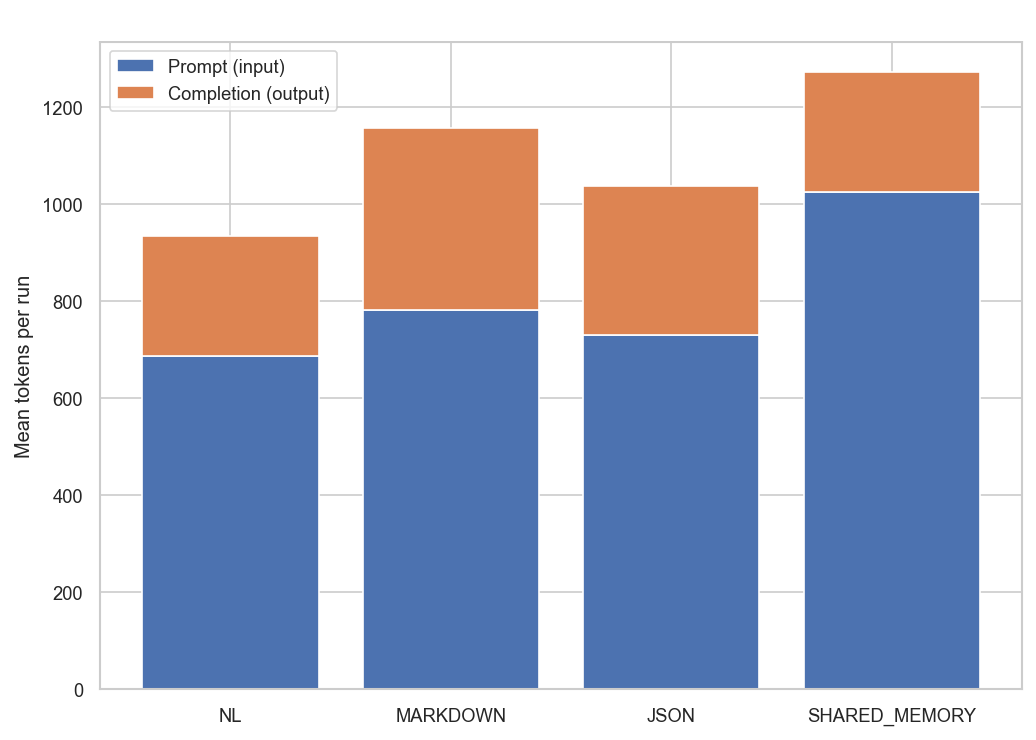
\includegraphics[width=0.86\linewidth]{report_fig5_input_vs_output.png}
\caption{Prompt-token and completion-token decomposition. Shared Memory mainly increases prompt tokens, while Markdown and JSON can increase completion tokens for open-ended news summaries.}
\label{fig:split}
\end{figure}

\subsection{RQ2: Effectiveness}

Completion quality is more domain-dependent than efficiency. The pooled protocol effect on completion is marginal and not significant at $\alpha=0.05$ (F=2.36, p=0.071), while domain is large and significant ($\eta^2=0.408$). This pooled result is not the full story: per-domain analyses show that protocol matters little for math but materially for reading and news.

\begin{table}[H]
\centering
\caption{Per-domain one-way ANOVA on completion score.}
\label{tab:domainanova}
\begin{tabular}{lrrrr}
\toprule
Domain & F & p-value & $\eta^2$ & Best vs worst Cohen's $d$ \\
\midrule
Math & 0.66 & 0.580 & 0.017 & 0.33 \\
Reading & 4.39 & 0.006 & 0.102 & 0.88 \\
News & 9.51 & $<0.001$ & 0.197 & 1.44 \\
\bottomrule
\end{tabular}
\end{table}

For math, no Tukey pair is significant. \MD has the highest mean exact-match score, 0.867, but \NL and \SM are close at 0.833 and \JS is 0.733. The small effect size suggests that once the final numeric answer is preserved, intermediate format is mainly a cost lever rather than a quality lever.

For reading, shared memory has the highest mean F1 at 0.556. Tukey HSD finds it significantly better than \MD (difference 0.208, p=0.003). The contrasts against \JS and \NL are positive but do not cross the family-wise threshold. This pattern suggests that the blackboard helps preserve exact spans or evidence for the integrator, while markdown structure can introduce paraphrase or verbosity that dilutes extractive answers.

For news, shared memory is significantly better than all other main protocols: +0.075 over \MD, +0.071 over \NL, and +0.051 over \JS. The effect is practically large despite the lower absolute ROUGE-scale values. News summaries reward retaining multiple facts, dates, quantities, and relations; a shared state snapshot gives the integrator more evidence to recover these facts.

\begin{figure}[H]
\centering
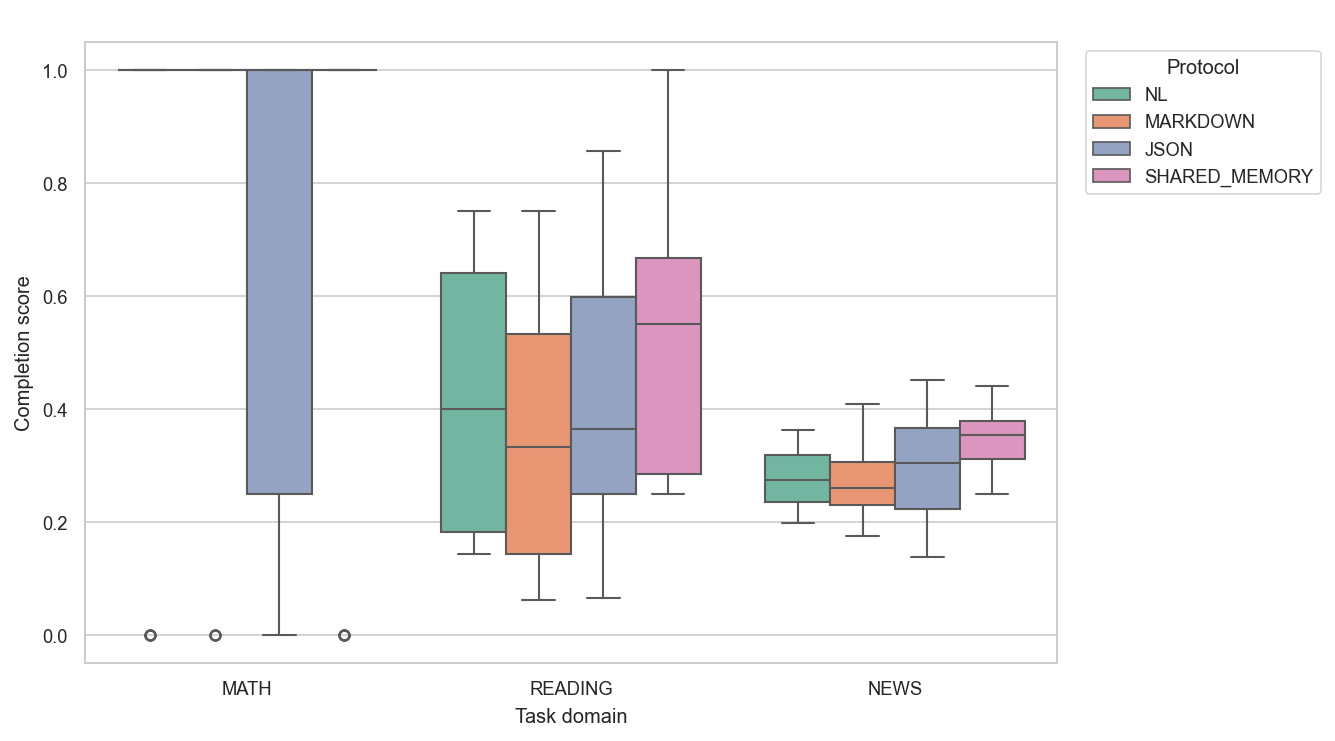
\includegraphics[width=0.96\linewidth]{report_fig2_completion_by_cell.png}
\caption{Completion score distributions by protocol and domain. Protocol effects are smallest for math and largest for news.}
\label{fig:completion}
\end{figure}

The interaction story is nuanced. The pooled protocol-by-domain interaction on completion is not statistically significant (F=1.43, p=0.203), but the per-domain effect sizes range from $\eta^2=0.017$ for math to $\eta^2=0.197$ for news. Thus, the formal interaction test is underpowered for completion at 30 observations per cell, while the descriptive pattern still matters for practitioner decisions. The observed global interaction effect is small ($\eta^2=0.014$), so this design is better powered for large per-domain effects than for weak global interactions. In contrast, the protocol-by-domain interaction on token cost is strongly significant, so the efficiency side of the trade-off clearly changes by domain.

\begin{figure}[H]
\centering
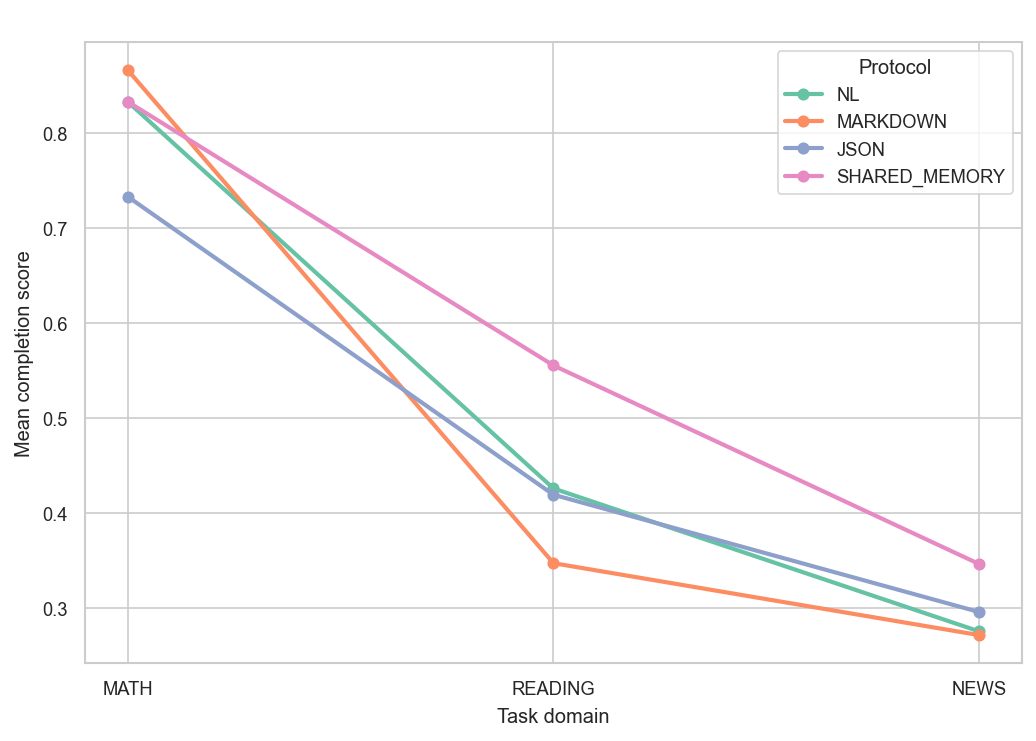
\includegraphics[width=0.86\linewidth]{report_fig3_interaction.png}
\caption{Interaction plot for completion score. The best protocol changes across domains: Markdown is narrowly best for math, while Shared Memory is best for reading and news.}
\label{fig:interaction}
\end{figure}

\subsection{Efficiency-Effectiveness Trade-off}

Figure~\ref{fig:pareto} summarizes the practical trade-off: lower tokens are better on the x-axis, higher completion is better on the y-axis. The Pareto frontier differs by domain.

\begin{figure}[H]
\centering
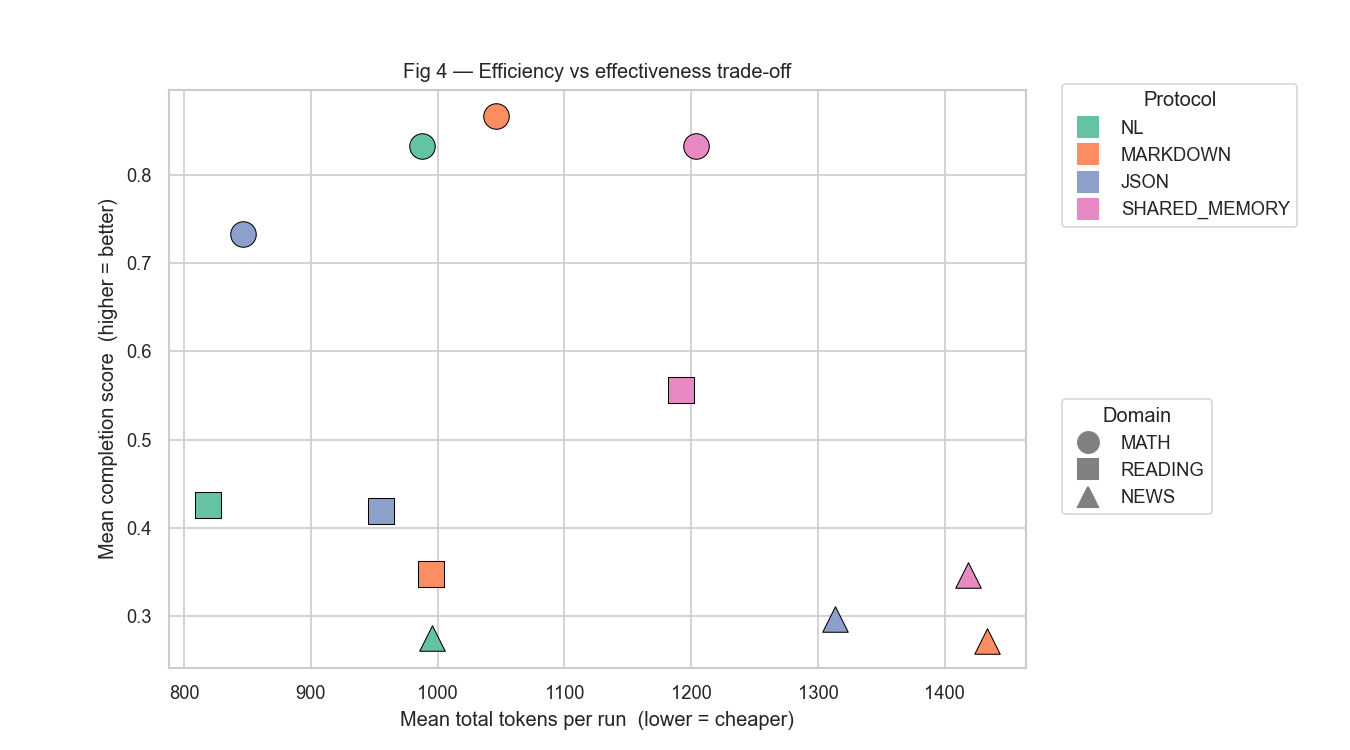
\includegraphics[width=0.95\linewidth]{report_fig4_pareto.png}
\caption{Efficiency-effectiveness trade-off. Shared Memory is often quality-favorable for text-heavy tasks, but it rarely minimizes token cost.}
\label{fig:pareto}
\end{figure}

The resulting recommendations are:

\begin{itemize}
  \item \textbf{Math.} Use \MD if completion is the primary goal; use \JS if token cost dominates. \SM is dominated by \NL because it has similar completion but higher token cost.
  \item \textbf{Reading.} Use \SM when exact-span preservation and quality matter; use \NL under tight token budgets.
  \item \textbf{News.} Use shared memory when factual recall matters; use \NL when cost dominates. \MD and \JS are dominated in the main grid because they cost more than \NL without matching shared-memory quality.
\end{itemize}

These recommendations are implemented in the FastAPI dashboard's recommendation panel, where users can compare live protocol runs against the offline experiment findings.

\subsection{Error Analysis}

The logged message data expose three main failure modes. First, JSON parsing is not a practical failure source in the main grid: \JS has 0 unrecoverable parse errors across 90 main runs, due to structured response formatting and one retry. Second, truncation is concentrated in math and markdown-like outputs. The main grid has 11 truncation-affected runs: 6 in \MD, 3 in \SM, 2 in \NL, and 0 in \JS. This supports the interpretation that markdown headings and bullets can inflate intermediate responses past the 256-token math budget. Third, shared memory occasionally over-retrieves stale context: the integrator has more information, but can copy plan text or earlier partial reasoning into the final response. That failure mode is less frequent than its reading/news benefits, but it explains why shared memory does not dominate math.

\subsection{Supplemental Ablation and Robustness Results}

The full mechanism-format ablation adds four protocols not in the main proposal grid: a relay default and three shared-memory format variants. The most important result is that blackboard state is expensive even when format is controlled. Across this supplemental grid, the relay default averages 824 tokens per run, while shared-memory NL averages 1,331, shared-memory JSON averages 1,676, and shared-memory markdown averages 1,733. Thus the overhead is not merely a property of JSON or markdown formatting; it is caused by repeatedly injecting accumulated shared state.

The ablation also warns against overclaiming that shared memory always improves quality. In the supplemental \texttt{gpt-4o-mini} ablation, \RD is best by mean completion in math, reading, and news. This does not contradict the main result that \SM is best among the proposal-defined protocols for reading and news. The main grid compares four course-proposal protocols exactly as deployed in the primary experiment. The ablation answers a different question: whether relay-vs-blackboard mechanism and surface format can be separated. Because \RD is a no-format relay baseline and the shared-memory variants add explicit format suffixes on top of blackboard state, the ablation is best interpreted as mechanism attribution for token cost, not as a replacement for the main inferential design.

The DeepSeek V4 Flash robustness run covers all eight protocols with 240 runs. It directionally confirms the overhead result: overall mean tokens are 752 for \RD, 869 for \NL, 1,018 for \JS, 1,166 for \MD, 1,278 for \SM, 1,333 for \SMN, 1,556 for \SMJ, and 1,946 for \SMM. However, the quality ranking changes: \RD is best for reading and news under this smaller DeepSeek subset, while several protocols tie at perfect math completion. The robust conclusion is therefore asymmetric. Token overhead mechanisms generalize more clearly than quality rankings, and protocol selection should be calibrated for the model family in production.

\section{Discussion}

The first hypothesis was that shared memory would incur higher overhead due to state serialization. The data strongly support this claim. In the main experiment, \SM is the most expensive pooled protocol and is more expensive than \NL in every domain. The supplemental ablation confirms that this is a blackboard-mechanism effect rather than a surface-format artifact.

The original expectation that JSON would be the lowest-token protocol is only partially supported. \JS is cheapest for math, where compact fields reduce both prompt and completion tokens. But \NL is cheaper for reading and news, likely because concise prose instructions and shorter responses avoid schema boilerplate. This is a useful practical correction: structured output can reduce ambiguity, but schema tokens are not free.

The second and third hypotheses concerned effectiveness and domain interaction. The strongest finding is not a universal protocol winner, but domain-specific trade-offs. For math, protocol choice mainly changes cost. For reading and news, shared memory often improves completion because it gives the integrator a richer evidence state. This comes at a substantial token premium. The pooled completion interaction is not significant, so the report avoids claiming a formal global interaction on quality; instead, it emphasizes per-domain effect sizes and the significant interaction on token cost.

For practitioners, the design rule is simple. Use lightweight relay protocols when the task has a compact final answer or when budget dominates. Use shared memory when downstream agents must preserve multiple pieces of evidence across a text-heavy task. Avoid assuming that one protocol is globally optimal; even the latest robustness run shows quality rankings can change with the base model.

\section{Demo and Reproducibility Artifacts}

The recommended demo is the FastAPI dashboard served by:

\begin{verbatim}
uvicorn fastapi_app:app --host 127.0.0.1 --port 8010 --http h11
\end{verbatim}

The dashboard includes an overview, experiment design view, protocol explorer, live protocol comparison, experiment database, results dashboard, and recommendations. The live demo uses local API credentials from \texttt{.env} or the environment; the browser does not ask the user to paste a key. The live runner is meant to demonstrate protocol overhead and domain-aware recommendations for the three benchmarked domains. Inputs outside these domains, such as code-generation requests, may be classified as \texttt{OTHER} and routed through the closest generic free-text path; those runs are useful for observing token and latency behavior, but they are not evidence of code-generation quality because this project does not yet include a code benchmark, code-specific prompts, or a code evaluator. The legacy Streamlit app remains available through \texttt{streamlit run app.py}, but the FastAPI dashboard is the polished presentation artifact.

The main experiment can be reproduced by installing \texttt{requirements.txt}, setting \texttt{OPENAI\_API\_KEY}, and executing:

\begin{verbatim}
jupyter nbconvert --to notebook --execute \
  Multi_Agent_Communication_Protocol_Study.ipynb \
  --output Multi_Agent_Communication_Protocol_Study.ipynb
\end{verbatim}

The supplemental runs are produced by the two underscore-prefixed runner scripts in the project root. The reported result set was generated under git commit \texttt{198a401}. The exact model, protocol list, max-token limits, sample counts, and evaluator descriptions are stored in \texttt{results/experiment\_config.json}.

\section{Limitations and Future Work}

The main limitation is scale. The primary grid uses 10 samples per domain and 3 repetitions per cell. This is enough to detect large efficiency effects and the larger per-domain completion effects in reading and news, but the observed global completion interaction is small ($\eta^2=0.014$) and underpowered at the current 30 observations per cell. A follow-up with at least 30 samples per domain, while preserving three repetitions and paired task identities across protocols, would better separate genuine domain-protocol interactions from sample noise.

Second, all main inferential results use one base model, \texttt{gpt-4o-mini}. The DeepSeek robustness run shows that token-cost mechanisms transfer better than quality rankings. Future work should repeat the full grid on several model families and report whether model capability changes the benefit of shared state.

Third, the current domains are intentionally narrow and relatively small. The math, reading, and news samples are enough for a controlled course-scale experiment, but they are simpler than the deeper multi-step tasks that motivate many real agent pipelines. Future work should add harder mathematical reasoning, longer document-analysis tasks, and code-generation or debugging benchmarks. These additions would test the broader hypothesis that better communication protocols can improve task completion on complex tasks, and may sometimes reduce tokens or latency by preventing downstream agents from re-deriving missing intermediate information.

Fourth, the protocol set is intentionally small. Future experiments should test XML, YAML, compact key-value formats, hybrid markdown-with-JSON protocols, and adaptive policies that switch format mid-pipeline based on confidence or budget.

Fifth, the evaluator design is automatic. Exact match, SQuAD F1, and ROUGE are reproducible, but they do not capture every semantic nuance. A future version should add a blinded human audit or LLM-as-judge validation for a stratified sample, while keeping the current automatic metrics as the primary reproducible outcome.

\section{Conclusion}

Communication protocol is not a cosmetic choice in multi-agent LLM systems. In our controlled three-agent pipeline, protocol choice explains a large share of token-cost variance, and shared memory consistently increases token cost because it serializes accumulated state into downstream prompts. Effectiveness is more domain-specific: protocol barely changes math completion, but shared memory improves reading and news quality in the main grid by preserving richer evidence for the final integrator.

The practical takeaway is a trade-off map rather than a single winner. Use JSON or natural-language relay when cost matters and answers are compact; use shared memory when text-heavy tasks require evidence retention; recalibrate the quality ranking when changing model families. The released framework, message logs, figures, and FastAPI dashboard make this recommendation reproducible and inspectable.

\appendix
\section{Rubric Alignment}

The final report addresses the course rubric as follows. Structure and format are covered through a conventional academic layout with cited related work, figures, tables, and an appendix. Depth of research is addressed in Section 2 through multi-agent frameworks, structured output, agent evaluation, and task-specific benchmark literature. Methodology is covered in Section 3 with the system model, protocols, data, evaluators, experimental design, and statistical analysis plan. Results and analysis are covered in Section 4 with ANOVA, Tukey interpretation, per-domain effect sizes, Pareto trade-offs, error analysis, and supplemental robustness results. Reproducibility and demo expectations are addressed in Section 6.

\begin{thebibliography}{12}

\bibitem{langgraph}
LangChain Team.
\newblock LangGraph: Building stateful, multi-actor applications with LLMs.
\newblock \url{https://github.com/langchain-ai/langgraph}, 2024.

\bibitem{autogen}
Q. Wu, G. Bansal, J. Zhang, Y. Wu, B. Li, E. Zhu, L. Jiang, X. Zhang, S. Zhang, J. Liu, A. H. Awadallah, R. W. White, D. Burger, and C. Wang.
\newblock AutoGen: Enabling next-gen LLM applications via multi-agent conversation.
\newblock arXiv preprint arXiv:2308.08155, 2023.

\bibitem{crewai}
J. Moura.
\newblock CrewAI: Framework for orchestrating role-playing autonomous AI agents.
\newblock \url{https://github.com/joaomdmoura/crewAI}, 2023.

\bibitem{toolformer}
T. Schick, J. Dwivedi-Yu, R. Dessi, R. Raileanu, M. Lomeli, L. Zettlemoyer, N. Cancedda, and T. Scialom.
\newblock Toolformer: Language models can teach themselves to use tools.
\newblock Advances in Neural Information Processing Systems, 36, 2023.

\bibitem{guided}
B. T. Willard and R. Louf.
\newblock Efficient guided generation for large language models.
\newblock arXiv preprint arXiv:2307.09702, 2023.

\bibitem{agentverse}
W. Chen, Y. Su, J. Zuo, C. Yang, C. Yuan, C.-M. Chan, H. Yu, Y. Lu, Y.-H. Hung, C. Qian, Y. Qin, X. Cong, R. Xie, Z. Liu, M. Sun, and J. Zhou.
\newblock AgentVerse: Facilitating multi-agent collaboration and exploring emergent behaviors in agents.
\newblock arXiv preprint arXiv:2308.10848, 2023.

\bibitem{agentbench}
X. Liu, H. Yu, H. Zhang, Y. Xu, X. Lei, H. Lai, Y. Gu, H. Ding, K. Men, K. Yang, S. Zhang, X. Deng, A. Zeng, Z. Du, C. Zhang, S. Shen, T. Zhang, Y. Su, H. Sun, M. Huang, Y. Dong, and J. Tang.
\newblock AgentBench: Evaluating LLMs as agents.
\newblock ICLR, 2024.

\bibitem{debate}
Y. Du, S. Li, A. Torralba, J. B. Tenenbaum, and I. Mordatch.
\newblock Improving factuality and reasoning in language models through multiagent debate.
\newblock arXiv preprint arXiv:2305.14325, 2023.

\bibitem{gsm8k}
K. Cobbe, V. Kosaraju, M. Bavarian, M. Chen, H. Jun, L. Kaiser, M. Plappert, J. Tworek, J. Hilton, R. Nakano, C. Hesse, and J. Schulman.
\newblock Training verifiers to solve math word problems.
\newblock arXiv preprint arXiv:2110.14168, 2021.

\bibitem{squad}
P. Rajpurkar, J. Zhang, K. Lopyrev, and P. Liang.
\newblock SQuAD: 100,000+ questions for machine comprehension of text.
\newblock EMNLP, 2016.

\bibitem{ie}
Z. Nasar, S. W. Jaffry, and M. K. Malik.
\newblock Information extraction from scientific articles: A survey.
\newblock Scientometrics, 117(3):1931--1990, 2018.

\bibitem{rouge}
C.-Y. Lin.
\newblock ROUGE: A package for automatic evaluation of summaries.
\newblock Proceedings of the ACL Workshop on Text Summarization Branches Out, pages 74--81, 2004.

\end{thebibliography}

\end{document}
